\section{Results}\label{sec:results}
 
\subsection{Overall Performance}
    Figure \ref{fig:OverallPerformance} shows the DCPT implementation preforming 10\% better than the included benchmark prefetchers. However, the RPT implementation achieves a speedup of only 2\%, slightly better than half of them.
    % Data
%----------------------------------------
\pgfplotstableread[row sep=\\,col sep=&]{
    prefetcher  & carT  \\
    This DCPT   & 1.10  \\
    This RPT    & 1.02  \\
    Tagged      & 1.01  \\
    SeqMiss     & 1.00  \\
    SeqAcc      & 1.01  \\
    RPT         & 1.06  \\
    DCPT-p      & 1.08  \\
    DCPT        & 1.05  \\
    AdapSeq    & 1.01  \\
    }\mydata

%Plot 
%----------------------------------------
\begin{figure}[!htb]
    \centering
    \begin{tikzpicture}
    \begin{axis}[
            ybar,
            ymin=.95,ymax=1.15,
            width = \textwidth/2,
            height = \textwidth/3,
            legend style={at={(0.5,1)},
                anchor=north,legend columns=-1},
            symbolic x coords={This DCPT, This RPT,Tagged,SeqMiss,SeqAcc,RPT,DCPT-p, DCPT, AdapSeq},
            xticklabel style={rotate=45},
            nodes near coords,
            nodes near coords align={vertical},
            xtick=data,
            %ylabel={Speedup},
        ]
        \addplot table[x=prefetcher,y=carT]{\mydata};
        
    \end{axis}
    \end{tikzpicture}
    
    \caption{Overall performance of different prefetchers}
    \label{fig:OverallPerformance}
\end{figure}

\subsection{Benchmarks}
    Figure \ref{fig:benchmarktest} shows how the RPT and DCPT prefetcher performs against each individual test. The DCPT prefetcher performs slightly worse on the \emph{twolf} test, but increases slightly until the \emph{wupwise} and \emph{ammp} tests, where it performs outstandingly well. RPT on the other hand has a negligible performance impact until run against the \emph{wupwise} and \emph{ammp} tests, where it performs slightly better.
    % Data
%----------------------------------------
\pgfplotstableread[row sep=\\,col sep=&]{
    bench   & DCPT & RPT  & nothing \\
    twolf   & 0.99 & 1.00 & 1.0 \\
    bzip2s  & 1.00 & 1.00 & 1.0 \\
    swim    & 1.01 & 0.99 & 1.0 \\
    bzip2g  & 1.03 & 1.01 & 1.0 \\
    bzip2p  & 1.04 & 1.01 & 1.0 \\
    art110  & 1.06 & 1.02 & 1.0 \\
    art470  & 1.06 & 1.02 & 1.0 \\
    apsi    & 1.09 & 1.01 & 1.0 \\
    applu   & 1.09 & 1.03 & 1.0 \\
    galgel  & 1.10 & 1.02 & 1.0 \\
    wupwise & 1.25 & 1.08 & 1.0 \\
    ammp    & 1.68 & 1.12 & 1.0 \\
    }\mydata

% Plot
%----------------------------------------
\begin{figure}[!htb]
\centering
\begin{tikzpicture}
    \begin{axis}[
            ybar,
            bar width=.1cm,
            width=\textwidth/2,
            height=\textwidth/3,
            %height=.5\textwidth/1,5,
            legend style={at={(0.5,1)},
                anchor=north,legend columns=-1},
            symbolic x coords={twolf, bzip2s, swim, bzip2g, bzip2p, art110, art470, apsi, applu, galgel, wupwise, ammp},
            xticklabel style={rotate=45},
            xtick=data,
            %nodes near coords,
            %nodes near coords align={vertical, rotate=90, anchor=west},
            ymin=.5,ymax=1.7,
            %ylabel={Speedup},
            %xlabel={Benchmark},
        ]
        \addplot table[x=bench,y=DCPT]   {\mydata};
        \addplot table[x=bench,y=RPT]    {\mydata};
        \addplot table[x=bench,y=nothing]{\mydata};
        \legend{DCPT, RPT, No Prefetch}
    \end{axis}
    \end{tikzpicture}
    \caption{Performance of DCPT vs RPT prefetchers}
    \label{fig:benchmarktest}
\end{figure}


\subsection{Statistics}
    Figure \ref{fig:statistics} shows the accuracy and coverage of the DCPT and the RPT prefetcher. These statistics can be calculated from equations (\ref{eq:coverage}) and (\ref{eq:accuracy}) which are explained in section \ref{sec:methodology}.
    % Data
%----------------------------------------
\pgfplotstableread[row sep=\\,col sep=&]{
    descr & DCPT & RPT            \\
    Accuracy     & 0.664  & 0.583 \\
    Coverage     & 0.471  & 0.10  \\
    }\mydata
%DCPT identified 2001231

% Plot
%----------------------------------------
\begin{figure}[!htb]
\centering
\begin{tikzpicture}
    \begin{axis}[
            ybar = 7pt,
            %bar width=.4cm,
            width=\textwidth/2,
            height=\textwidth/3,
            legend pos = north east,
            symbolic x coords={Accuracy, Coverage},
            xticklabel style={rotate=45},
            xtick=data,
            enlarge x limits = 0.7,
            nodes near coords,
            nodes near coords align={vertical},
            ymin=0, ymax=0.8,
            %ylabel={Speedup},
            %xlabel={Benchmark},
        ]
        \addplot table[x=descr,y=DCPT]{\mydata};
        \addplot table[x=descr,y=RPT]{\mydata};
        \legend{DCPT, RPT}
    \end{axis}
    \end{tikzpicture}
    \caption{Statistics for DCPT and RPT prefetchers}
    \label{fig:statistics}
\end{figure}


\subsection{Cache Size}
    Figure \ref{fig:cachesize} shows how the different implementations performed when the L2 cache size was changed. Because the speedup value is given in reference to a 1MB L2 cache, the relative speedups of using no prefetcher is also given. They were tested with a 1MB, 2MB, 4MB, 8MB, and 16MB L2 cache size. 
    \begin{figure}[!htb]
    \centering
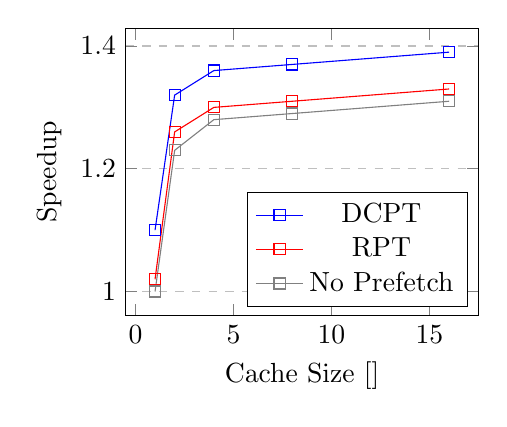
\begin{tikzpicture}
\begin{axis}[
    xlabel={Cache Size \SI{}{[\mega\byte]}},
    ylabel={Speedup},
    %xtick={0,1 ,2, 4, 8, 16},
    %ytick={0,0.5,1,1.5, 2},
    %nodes near coords,
    %nodes near coords align={vertical},
    legend pos=south east,
    ymajorgrids=true,
    grid style=dashed,
    width=\textwidth/2,
]
%DCPT
\addplot[
    color=blue,
    mark=square,
    ]
    coordinates {
    (1,1.1)(2,1.32)(4,1.36)(8,1.37)(16, 1.39)
    };
    
%RPT
\addplot[
    color=red,
    mark=square,
    ]
    coordinates {
    (1,1.02)(2,1.26)(4, 1.30)(8, 1.31)(16, 1.33)
    };
    
%No Prefetch
\addplot[
    color=gray,
    mark=square,
    ]
    coordinates {
    (1,1.0)(2,1.23)(4,1.28)(8,1.29)(16, 1.31)
    };

    \legend{DCPT, RPT, No Prefetch}
    
\end{axis}
\end{tikzpicture}
    \caption{Speedups compared to 1MB L2 cache with no prefetching}
    \label{fig:cachesize}
\end{figure}
    
\subsection{Delta Size}
    Figure \ref{fig:deltaEntries} shows how changing the amount of deltas per entry effects the relative speed up of the DCPT algorithm. Because RPT does not have a number of delta entries, it is not included in this graph.
    \begin{figure}[!htb]
    \centering
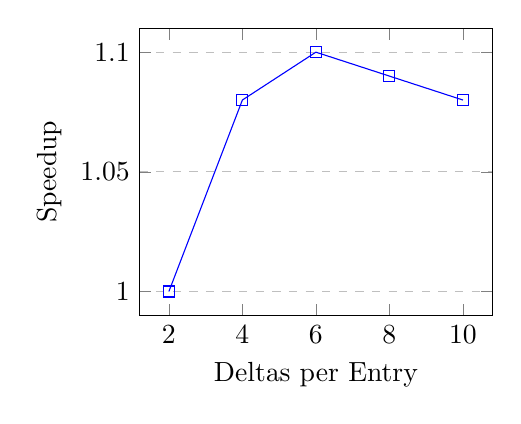
\begin{tikzpicture}
\begin{axis}[
    xlabel={Deltas per Entry},
    ylabel={Speedup},
    %xtick={0,1 ,2, 4, 8, 16},
    %ytick={0,0.5,1,1.5, 2},
    %nodes near coords,
    %nodes near coords align={vertical},
    legend pos=south east,
    ymajorgrids=true,
    grid style=dashed,
    width=\textwidth/2,
]
%DCPT
\addplot[
    color=blue,
    mark=square,
    ]
    coordinates {
    (2,1.00)(4,1.08)(6,1.1)(8,1.09)(10,1.08)
    };
    
    %\legend{DCPT, No Prefetch}
    
\end{axis}
\end{tikzpicture}
    \caption{Speedup of the DCPT algorithm with different amounts of deltas in each entry.}
    \label{fig:deltaEntries}
\end{figure}